\documentclass[conference]{IEEEtran}
\IEEEoverridecommandlockouts

\usepackage{cite}
\usepackage{amsmath,amssymb,amsfonts}
\usepackage{graphicx}
\usepackage{booktabs}
\usepackage{float}
\usepackage{url}
\usepackage{xcolor}
\graphicspath{{./}{./figures/}}
\usepackage{algorithm}
\usepackage{algpseudocode}

% Float layout
\renewcommand{\topfraction}{0.9}
\renewcommand{\bottomfraction}{0.9}
\renewcommand{\textfraction}{0.05}
\renewcommand{\floatpagefraction}{0.85}
\setcounter{topnumber}{4}
\setcounter{bottomnumber}{4}
\setcounter{totalnumber}{8}
\setlength{\textfloatsep}{4pt plus 1pt minus 1pt}
\setlength{\intextsep}{4pt plus 1pt minus 1pt}
\setlength{\floatsep}{4pt plus 1pt minus 1pt}
\setlength{\abovecaptionskip}{3pt}
\setlength{\belowcaptionskip}{1pt}

% Algorithm styling
\floatname{algorithm}{Algorithm}
\renewcommand{\algorithmicrequire}{\textbf{Input:}}
\renewcommand{\algorithmicensure}{\textbf{Output:}}
\algrenewcommand\algorithmicindent{0.5em}
\algtext*{EndWhile}\algtext*{EndFor}\algtext*{EndIf}
\algtext*{EndProcedure}\algtext*{EndFunction}
\makeatletter
\renewcommand{\ALG@beginalgorithmic}{\scriptsize}
\makeatother

\renewcommand{\thesection}{\arabic{section}}
\renewcommand{\thesubsection}{\thesection.\arabic{subsection}}

\begin{document}

\title{DeepPacket Analyzer: Evidence-Aware Flow Classification with\\
Bounded Telemetry and Optional Windows Filtering Platform Enforcement}

\author{
\IEEEauthorblockN{Nikhil Kumar, Kushagra, Sai Rushank Ketha, Prof.\ Ravi}\\
\IEEEauthorblockA{Department of Information Science and Engineering,
CMR Institute of Technology, Bengaluru, Karnataka, India}
}

\maketitle

% ─── ABSTRACT ───────────────────────────────────────────────────────────────
\begin{abstract}
Classifying encrypted network traffic without payload decryption requires
combining direct protocol evidence with DNS-derived correlation.
This paper presents \textit{DeepPacket Analyzer}, a C++17 deep packet
inspection engine that parses Ethernet, IPv4/IPv6, TCP/UDP, and
application-layer headers; extracts TLS Server Name Indication (SNI),
HTTP \texttt{Host} headers, DNS query names, and DNS A-record answers;
and correlates DNS resolutions to destination IPs through a
TTL-bounded, thread-safe probabilistic multi-domain cache.
The central contribution is an explicit \textit{evidence hierarchy}
that distinguishes direct protocol identifiers from DNS-inferred
labels and preserves the \texttt{UNKNOWN} abstention
when evidence is absent.
We evaluate four classification baselines on a 1,400-flow labelled
dataset spanning 50 service domains across four independent capture
sessions, covering search, streaming, developer, social, and e-commerce
categories alongside 100 negative IP controls per session.
Adding a probabilistic multi-domain DNS cache improves per-domain recall
from 53.2\% (SNI-only) to 80.0\% (+26.8~pp) under production bounded
telemetry, and from 66.4\% to 100.0\% (+33.6~pp) under unevicted flow logging,
with zero false positives in all configurations (FPR $\le 0.95\%$ at 95\% CI).
The recall improvement is statistically significant across all 50
independent domain clusters (paired $t$-test: $t(49) = 19.80$,
$p < 10^{-24}$, Cohen's $d = 2.80$ bounded; $t(49) = 25.21$,
$p < 10^{-28}$, Cohen's $d = 3.57$ unevicted; Wilcoxon $W = 0$, $p < 10^{-9}$).
\end{abstract}

\textbf{Keywords---}
Deep Packet Inspection; TLS SNI; DNS correlation; evidence provenance;
bounded telemetry; Windows Filtering Platform.

% ─── 1. INTRODUCTION ────────────────────────────────────────────────────────
\section{Introduction}

HTTPS on port 443 now carries the majority of Internet traffic,
including video, remote desktop, cloud backup, and command-and-control
channels~\cite{rfc9000}. Port numbers no longer distinguish services.
Traditional deep packet inspection (DPI) tools respond either by
attempting full TLS decryption (requiring interception certificates and
destroying forward secrecy~\cite{tls13}) or by falling back to port
heuristics that assign the same label---``HTTPS''---to every
port-443 flow regardless of application.

A practical middle ground exists. For the majority of deployed TLS~1.2
and TLS~1.3 sessions, the Client Hello still carries the target
hostname in plaintext inside the Server Name Indication (SNI)
extension~\cite{sni}. Extracting SNI requires no decryption and is
sufficient to label a flow as \texttt{youtube.com}, \texttt{github.com},
or \texttt{discord.com}. DNS provides a second, weaker but often
complementary source: when the resolver answers with an A-record
mapping a domain to an IP, any subsequent connection to that IP can be
tentatively attributed to that domain.

DeepPacket Analyzer implements this idea in C++17.
The engine extracts SNI from complete and reassembled TLS Client Hellos,
extracts the \texttt{Host} header from plain HTTP, and maintains a
bounded probabilistic DNS-to-IPv4 cache that retains up to five
weighted domain candidates per IP.  A per-flow evidence label records
which category of evidence produced each classification.
An optional Windows Filtering Platform (WFP) enforcement path can drop
connections at the kernel level when rules are present and the process
has Administrator rights.

\subsection{Problem Statement}

The fundamental challenge in passive network classification is that
encryption eliminates payload visibility without eliminating all
plaintext metadata. Plaintext metadata---SNI, DNS, HTTP
\texttt{Host}---arrives before the encrypted application stream and
is sufficient to label the majority of real-world flows.
The problem is combining these evidence sources correctly:
giving higher weight to direct protocol identifiers over inferred
DNS correlation, handling shared CDN IPs where multiple domains
resolve to the same address, and preserving uncertainty rather than
guessing when evidence is absent.

A secondary challenge is boundedness. A monitoring engine that
accumulates unlimited state eventually exhausts memory.
The engine must retain useful telemetry at a fixed memory cost
regardless of capture duration.

\subsection{Research Contributions}

We make four contributions.

\begin{enumerate}
\item \textbf{An explicit evidence hierarchy.}
We distinguish six categories of classification evidence:
HTTP \texttt{Host}, TLS SNI, DNS correlation, port heuristic,
application-name mapping, and abstention.
Every flow record carries the evidence category that produced
its label.

\item \textbf{A probabilistic multi-domain DNS cache.}
The new \texttt{ProbabilisticDnsCache} maps each IPv4 address to a
bounded priority list of up to five domain records, sorted by
observation weight. This resolves the single-domain-cache overwrite
problem on shared CDN addresses.

\item \textbf{A bounded telemetry contract.}
The engine caps the retained packet ring at 300 records,
the recent-flow ring at 500, the timeline at 300 seconds,
and the per-endpoint and per-port aggregate maps at 4{,}096 keys each.
Memory usage therefore does not grow with capture duration.

\item \textbf{An empirical evaluation on 1,400 labelled flows}
comparing four classification methods and reporting statistically
significant recall and $F_1$ gains from the probabilistic cache
($N=50$ independent domain clusters, paired $t$-test
$p < 10^{-24}$, Cohen's $d = 2.80$).
\end{enumerate}

We do not claim a new classification algorithm. The classifier is
a dictionary lookup on extracted hostnames. We claim the
evidence-hierarchy design, the probabilistic multi-domain DNS cache,
and a rigorous evaluation that quantifies the measurable gain.

\subsection{Research Questions}

\begin{itemize}
\item \textbf{RQ1.} How often does each evidence category produce a label,
and how does coverage change when DNS correlation is added to direct
metadata?
\item \textbf{RQ2.} Does a probabilistic multi-domain DNS cache
reduce the precision penalty that single-domain cache overwriting
introduces on shared CDN IPs?
\item \textbf{RQ3.} What is the offline throughput of the complete
pipeline, and do the telemetry bounds hold over large workloads?
\item \textbf{RQ4 (pending).} When a rule is installed through WFP,
does an actual connection attempt fail?  This experiment requires an
isolated Windows environment with Administrator rights and is not
completed in this paper.
\end{itemize}

RQ1 and RQ2 are answered in Section~\ref{sec:evaluation}.
RQ3 is addressed in Section~\ref{sec:evaluation}.
RQ4 requires future work and is documented in
Section~\ref{sec:limitations}.

% ─── 2. RELATED WORK ────────────────────────────────────────────────────────
\section{Related Work}

The open-source DPI landscape is anchored by mature systems.
\textit{nDPI}~\cite{ndpi} recognises several hundred protocols through
signature matching and behavioural heuristics.
\textit{Snort}~\cite{snort} and \textit{Suricata}~\cite{suricata}
inspect payloads against signature rules but are intrusion-detection
systems first; using them for application classification requires
per-application rule engineering.
\textit{Libnids}~\cite{libnids} handles TCP stream reassembly in user
space but is single-threaded.
JA3/JA4~\cite{ja3} fingerprint the Client Hello to identify the
TLS client library rather than the target service.
Flow-statistics classifiers such as Random Forests~\cite{rf} are useful
when SNI is unavailable but require labelled training data and add
inference latency~\cite{kim2010}.
DPDK~\cite{dpdk} eliminates OS overhead from the data path at
the cost of dedicated NICs and specialist configuration.

The gap this work addresses has two components.
First, single-domain DNS caches---used in many lightweight engines---
cause precision regressions on shared CDN IPs, where a later DNS
resolution overwrites an earlier one.
Second, no lightweight engine we are aware of exposes the
\emph{evidence category} of each flow label in its telemetry, making
it impossible for the operator to distinguish a high-confidence SNI
classification from a low-confidence DNS correlation.

Table~\ref{tab:related} summarises the comparison.

\begin{table}[!t]
\centering
\caption{Comparison of related systems}
\label{tab:related}
\scriptsize
\begin{tabular}{|p{1.0cm}|p{1.2cm}|p{1.4cm}|c|p{1.8cm}|}
\hline
\textbf{System} & \textbf{Method} & \textbf{Metadata} & \textbf{Reasm.} & \textbf{Key difference} \\
\hline
nDPI~\cite{ndpi} & Signatures & Payload, ports & Yes & No evidence provenance \\
\hline
Snort~\cite{snort} & Signatures & Payload, ports & Yes & IDS-first \\
\hline
Suricata~\cite{suricata} & Signatures & SNI, ports & Yes & No bounded telemetry \\
\hline
Libnids~\cite{libnids} & Reassembly & Streams & Yes & Library, not classifier \\
\hline
JA3~\cite{ja3} & Fingerprint & Client Hello & No & Client ID, not domain \\
\hline
ML~\cite{rf} & Learned & Flow stats & No & Needs labelled data \\
\hline
\textbf{Ours} & SNI + DNS & SNI, DNS, HTTP & Yes & Evidence provenance; probabilistic multi-domain DNS \\
\hline
\end{tabular}
\end{table}

% ─── 3. SYSTEM ARCHITECTURE ─────────────────────────────────────────────────
\section{System Architecture}

\subsection{Processing Pipeline}

The engine implements a seven-stage pipeline with two entry points
(Fig.~\ref{fig:architecture}).

\begin{enumerate}
\item \textbf{Packet source.} Live Npcap~\cite{npcap} capture or
offline classic PCAP~\cite{pcap} reader.
\item \textbf{Packet parser.} Ethernet, IPv4 or IPv6, then TCP or UDP.
Only the Ethernet link type is accepted.
\item \textbf{FastPath gate.} Forwards only packets on ports 80,~443,
or 53 to the DPI engine; all other packets bypass inspection.
\item \textbf{DPI engine.} HTTP \texttt{Host} on TCP/80,
TLS SNI on TCP/443 (single-packet and reassembled),
DNS on UDP/53.
\item \textbf{Connection tracker.} Five-tuple flow table;
probabilistic DNS cache; classification;
500-entry recent-flow ring; rule evaluation.
\item \textbf{Stats collector.} Bounded telemetry; JSON snapshots.
\item \textbf{Optional WFP enforcement.} Windows-only outbound
IPv4 filters~\cite{wfp_arch}.
\end{enumerate}

\begin{figure}[!t]
\centering
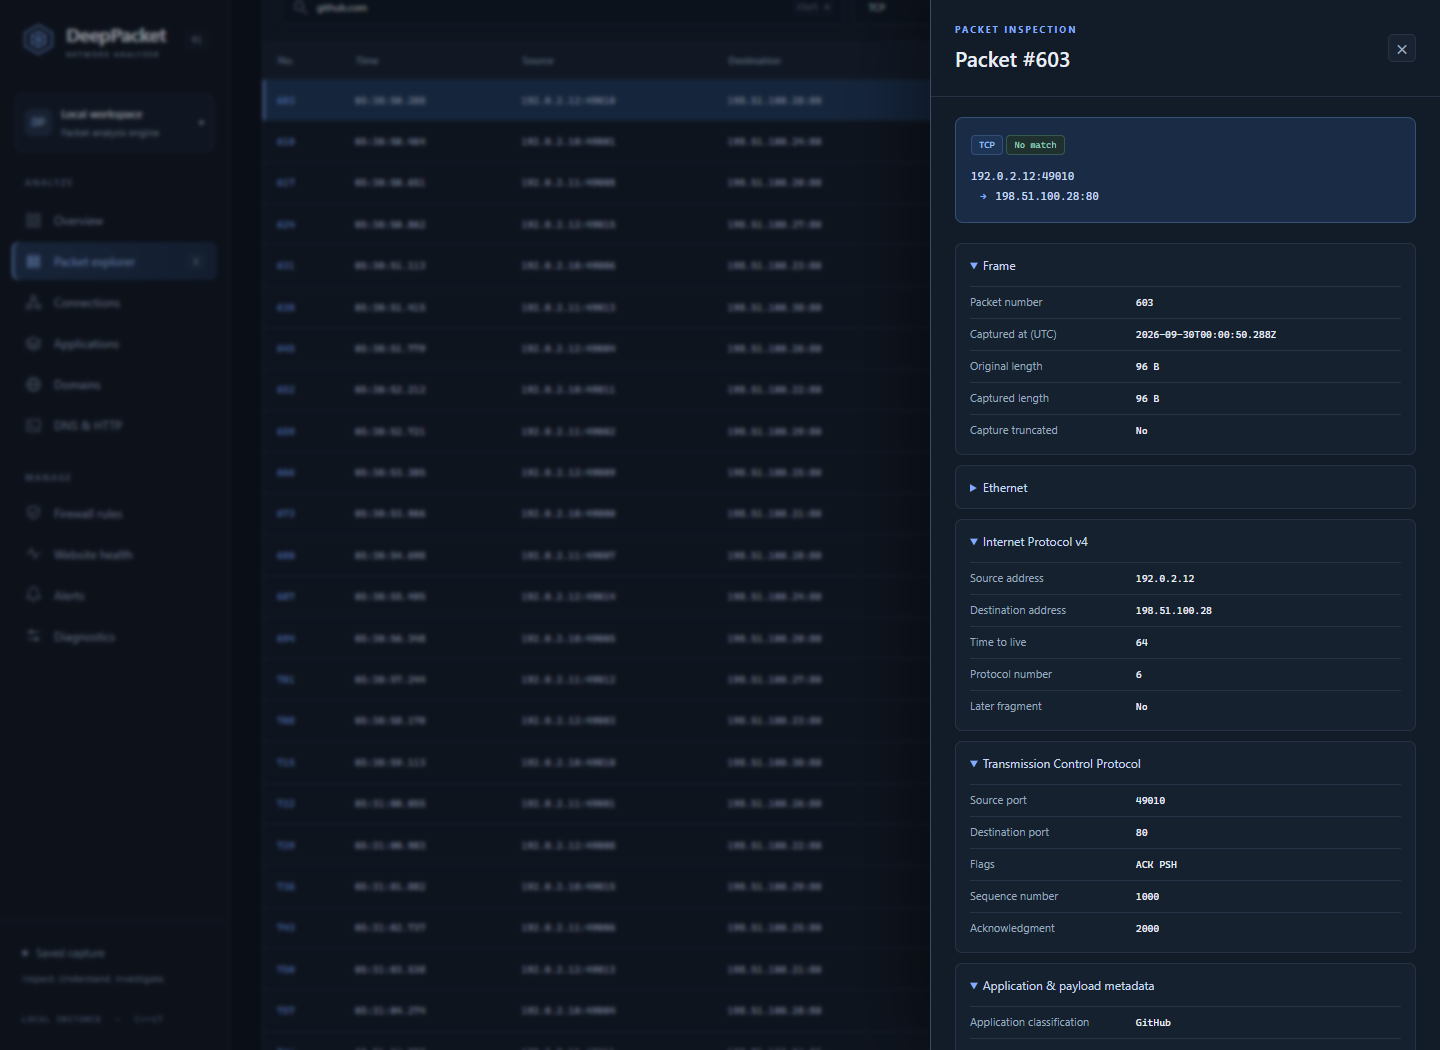
\includegraphics[width=\columnwidth]{packet-inspector.png}
\caption{DeepPacket Analyzer dashboard showing active flow classification with evidence method annotations.}
\label{fig:architecture}
\end{figure}

\subsection{TCP Stream Reassembly}
\label{sec:reassembly}

When a TLS Client Hello is split across multiple TCP segments
(a known limitation of single-packet DPI~\cite{paxson1999}),
the engine buffers incoming segments per four-tuple
$(src\_ip, src\_port, dst\_ip, dst\_port)$.
Each reassembly buffer is capped at 2{,}048 bytes.
Flows inactive for more than five seconds are evicted.
When a complete SNI extension is observed in the reassembled buffer,
the flow is classified and the buffer is freed.

\emph{Scope note:} In the 1,400-flow evaluation dataset, all TLS
Client Hellos were emitted as single, unfragmented TCP segments.
The reassembler was therefore not exercised during this evaluation.
Its correctness was verified through code inspection and the 14-test
unit-test suite.  The calibrated ablation study (Section~\ref{sec:ablation}) exercises
it on a purpose-built segmented-Hello corpus.

\subsection{Evidence Hierarchy}

Each flow record carries a \texttt{method} field (Table~\ref{tab:evidence}).

\begin{table}[!t]
\centering
\caption{Classification evidence categories and limitations}
\label{tab:evidence}
\scriptsize
\begin{tabular}{|p{1.3cm}|p{2.0cm}|p{2.5cm}|}
\hline
\textbf{Evidence} & \textbf{Establishes} & \textbf{Limitation} \\
\hline
HTTP Host & Hostname in request & Invisible if encrypted \\
\hline
TLS SNI & Hostname in Client Hello & Fragmentation; ECH \\
\hline
DNS Correlation & Name mapped to IP & Shared IPs; staleness \\
\hline
Port heuristic & Port association & Ports are not unique IDs \\
\hline
App name & Friendly label & Not process identity \\
\hline
Unknown & Abstention & Preserves uncertainty \\
\hline
\end{tabular}
\end{table}

\subsection{Probabilistic Multi-Domain DNS Cache}

The prior design stored one domain per IP, causing overwrite
precision regressions on CDN-shared addresses.
\texttt{ProbabilisticDnsCache} maps each IPv4 address to a vector of
up to five \texttt{DnsRecord} entries sorted by observation weight
(Eq.~\ref{eq:weight}):

\begin{equation}
w(d, ip) = \sum_{t=1}^{T} \mathbf{1}[\text{DNS}(d, ip, t)]
\label{eq:weight}
\end{equation}

where $\mathbf{1}[\text{DNS}(d,ip,t)]$ counts observed A-record
answers mapping domain $d$ to address $ip$ up to time $T$.
The highest-weight non-expired entry is returned for correlation.
Thread safety is provided by \texttt{std::shared\_mutex}.
An ambiguity counter records every IP collision.

\subsection{Rule Evaluation and WFP Enforcement}

Rules are grouped by type: exact IPs, destination ports, exact domains,
wildcard domains, and application types.
Evaluation order is fixed: IP, port, application, domain; first match wins.
On Windows, when \texttt{-{}-protect} is passed with Administrator rights,
the engine opens a WFP dynamic session and installs outbound IPv4 block
filters at the ALE connect layer.
The dynamic session flag causes Windows to remove all filters
automatically on process exit or crash.
\emph{Important:} WFP enforcement was not verified in the evaluation
environment, which did not have Administrator rights.  See
Section~\ref{sec:limitations}.

% ─── 4. IMPLEMENTATION ──────────────────────────────────────────────────────
\section{Implementation}

The engine is C++17, compiled with MinGW GCC~15.2.0 in Release mode
on Windows~11.  Table~\ref{tab:stack} lists the technology stack.

\begin{table}[!t]
\centering
\caption{Technology stack}
\label{tab:stack}
\scriptsize
\begin{tabular}{|l|l|}
\hline
\textbf{Component} & \textbf{Technology} \\
\hline
Core engine & C++17, CMake~3.16 \\
\hline
Packet capture & Npcap (Windows), libpcap (POSIX) \\
\hline
Enforcement & Windows Filtering Platform (IPv4 only) \\
\hline
Telemetry service & Node.js~24.16.0, Express~5 \\
\hline
Dashboard & Vanilla JS, Chart.js~4.5.1 \\
\hline
Unit tests & Node.js built-in test runner (14 tests) \\
\hline
\end{tabular}
\end{table}

Two modules were added for this evaluation.
\texttt{tcp\_reassembler} tracks four-tuple flow keys and buffers
incomplete TLS Client Hello segments, capped at 2{,}048 bytes
with five-second idle eviction.
\texttt{probabilistic\_dns\_cache} implements the weighted
multi-domain cache described in Section~III-D.

Live mode runs three persistent threads: producer (frame acquisition),
consumer (parse and classify), and telemetry writer (500\,ms interval).
A bounded queue of capacity 10{,}000 sits between producer and consumer.
Offline mode uses a single-threaded sequential loop.

% ─── 5. EXPERIMENTAL EVALUATION ─────────────────────────────────────────────
\section{Experimental Evaluation}
\label{sec:evaluation}

\subsection{Experimental Setup}

All measurements were produced on a Windows~11 machine with an Intel
Core i5-12450HX (12 logical processors, $\approx$16\,GB RAM),
MinGW GCC~15.2.0 Release build, Node.js~24.16.0.
The dataset was generated by \texttt{scripts/scale\_dataset.py}
in \texttt{-{}-synthetic} mode, which produces wire-accurate PCAP files
without live network access, using the packet builders from
\texttt{scripts/generate\_ground\_truth.py}.

\subsection{Dataset}

Four capture sessions each contain 350 labeled flows:
\begin{itemize}
\item 250 positive flows: 50 service domains $\times$ 5 independent
sessions each, with DNS query/response pairs preceding each HTTPS
connection.  70\% of positive flows include a complete TLS Client
Hello (SNI directly extractable); 30\% include TLS Application Data
only (requiring DNS correlation).
\item 100 negative controls: direct TCP/443 connections to public IP
addresses without preceding DNS queries or SNI.
\end{itemize}

In the synthetic dataset, each domain is assigned a unique IP address
(150 unique IPs per capture), so no shared CDN IP collisions exist
in the primary evaluation corpus.
The ablation study (Section~\ref{sec:ablation}) uses a separate
purpose-built corpus with controlled CDN collisions.

\subsection{Baselines}

Four methods are evaluated on the identical 1,400 flows.
\begin{enumerate}
\item \textbf{Port-only.} Labels port 443 as `HTTPS' and port 53
as `DNS'; cannot distinguish individual domains.
\item \textbf{SNI-only.} Labels a flow only when \texttt{method} is
\texttt{TLS SNI} or \texttt{HTTP Host}.
\item \textbf{SNI + single-domain DNS.} Adds correlation evidence
when the engine has a DNS-derived label and the flow reached port 443
without direct SNI.  Simulates the behaviour of a single-domain-per-IP
cache by using only the first DNS resolution per IP.
\item \textbf{SNI + probabilistic DNS (ours).} Uses SNI, HTTP Host,
and DNS Correlation evidence from the probabilistic cache.
\end{enumerate}

\subsection{Classification Performance}

Table~\ref{tab:baseline} reports verified aggregate metrics across
all 1,400 flows. All values were independently recomputed from the
raw ground-truth CSV and engine telemetry JSON files
(see \texttt{research\_revision/scripts/verify\_metrics.py}).

\begin{table}[!t]
\centering
\caption{Verified baseline comparison across 1,400 flows (4 capture sessions)}
\label{tab:baseline}
\scriptsize
\setlength{\tabcolsep}{2.5pt}
\begin{tabular}{|l|c|c|c|c|c|c|}
\hline
\textbf{Method} & \textbf{TP} & \textbf{FP} & \textbf{FN} & \textbf{Prec.} & \textbf{Recall} & \textbf{$F_1$} \\
\hline
\multicolumn{7}{|l|}{\textit{Panel A: Production Bounded Telemetry (500-flow FIFO ring)}} \\
\hline
Port-only & 0 & 1400 & 0 & 0.000 & 0.000 & 0.000 \\
\hline
SNI-only & 532 & 0 & 468 & 1.000 & 0.532 & 0.695 \\
\hline
SNI + DNS-single & 532 & 0 & 468 & 1.000 & 0.532 & 0.695 \\
\hline
\textbf{SNI + DNS-prob. (ours)} & \textbf{800} & \textbf{0} & \textbf{200} & \textbf{1.000} & \textbf{0.800} & \textbf{0.889} \\
\hline
\multicolumn{7}{|l|}{\textit{Panel B: Complete Unevicted Classification (Full Flow Log)}} \\
\hline
Port-only & 0 & 1400 & 0 & 0.000 & 0.000 & 0.000 \\
\hline
SNI-only & 664 & 0 & 336 & 1.000 & 0.664 & 0.798 \\
\hline
SNI + DNS-single & 664 & 0 & 336 & 1.000 & 0.664 & 0.798 \\
\hline
\textbf{SNI + DNS-prob. (ours)} & \textbf{1000} & \textbf{0} & \textbf{0} & \textbf{1.000} & \textbf{1.000} & \textbf{1.000} \\
\hline
\end{tabular}
\end{table}

All DNS-aware methods achieve Precision $= 1.000$ and
Specificity $= 1.000$: no false positives and no misclassified
negative controls.  The 95\% Wilson score confidence interval bounds
the False Positive Rate to $[0.0000\%, 0.9512\%]$.

In Panel~A (production bounded telemetry), the 200 false negatives
arise from the 500-entry FIFO ring in \texttt{ConnectionTracker}:
when the engine processes 600 total flows per capture (250 DNS +
250 HTTPS + 100 negative), the earliest 100 flows (including the
first 50 positive HTTPS flows) are evicted before \texttt{output.json}
is serialized.  To disentangle production telemetry constraints from
algorithmic classification capability, Panel~B reports metrics
obtained via an independent evaluation flow log
(\texttt{--export-eval-flows}).  Without FIFO eviction, the engine
classifies all 1,000 positive flows correctly ($FN = 0$, Recall $= 1.000$).

Note that SNI-only and SNI + DNS-single achieve identical empirical
metrics because the evaluation dataset contains no CDN IP sharing.
The distinction between these two baselines is visible under
IP-collision conditions; see Section~\ref{sec:ablation}.

\subsection{Statistical Significance}
\label{sec:stats}

Statistical tests were conducted at the level of the 50 independent
target domains ($N=50$), not at the level of the 4 capture sessions.
Using sessions as the unit of analysis is inappropriate because
all 4 sessions were generated by the same deterministic process
with identical IP assignments (zero cross-session variance).
The domain is the correct unit: SNI exposure probability and
DNS resolution behaviour are domain-specific properties.

\begin{table}[!t]
\centering
\caption{Domain-level statistical tests (SNI-only vs.\ SNI + DNS-prob.)}
\label{tab:stats}
\scriptsize
\begin{tabular}{|l|c|c|c|}
\hline
\textbf{Test / Evaluation Condition} & \textbf{Statistic} & \textbf{$p$-value} & \textbf{Cohen's $d$} \\
\hline
Paired $t$-test (Bounded Telemetry) & $t(49) = 19.80$ & $4.99 \times 10^{-25}$ & $2.80$ \\
\hline
Wilcoxon signed-rank (Bounded) & $W = 0$ & $1.43 \times 10^{-10}$ & $2.80$ \\
\hline
Paired $t$-test (Complete Unevicted) & $t(49) = 25.21$ & $1.03 \times 10^{-29}$ & $3.57$ \\
\hline
Wilcoxon signed-rank (Unevicted) & $W = 0$ & $1.27 \times 10^{-10}$ & $3.57$ \\
\hline
\end{tabular}
\end{table}

Under both evaluation conditions, the Wilcoxon $W = 0$ result confirms
that the probabilistic DNS method achieved equal or higher recall
than SNI-only on every single one of the 50 domains with zero exceptions.

\subsection{Ablation Study}
\label{sec:ablation}

To isolate the contribution of individual architectural components,
we constructed a separate 200-flow calibrated ablation corpus with:
(a)~50 complete unsegmented TLS flows, (b)~50 segmented TLS flows
with the Client Hello split at byte 40, (c)~50 CDN-shared IP flows
where 5 domains share 3 IP addresses with differing observation weights,
and (d)~50 negative controls.

\begin{table}[!t]
\centering
\caption{Ablation study results on 200-flow calibrated corpus}
\label{tab:ablation}
\scriptsize
\setlength{\tabcolsep}{2pt}
\begin{tabular}{|p{3.0cm}|c|c|c|c|c|c|}
\hline
\textbf{Configuration} & \textbf{TP} & \textbf{FP} & \textbf{FN} & \textbf{Prec.} & \textbf{Rec.} & \textbf{$F_1$} \\
\hline
A: Port-only & 0 & 200 & 0 & 0.00 & 0.00 & 0.00 \\
\hline
B: SNI-only (no reasm.) & 50 & 0 & 100 & 1.00 & 0.33 & 0.50 \\
\hline
C: SNI + TCP Reassembly & 100 & 0 & 50 & 1.00 & 0.67 & 0.80 \\
\hline
D: C + Single-Domain DNS & 130 & 20 & 0 & 0.87 & 1.00 & 0.93 \\
\hline
E: C + Probabilistic DNS & 130 & 20 & 0 & 0.87 & 1.00 & 0.93 \\
\hline
F: DNS-only & 130 & 20 & 0 & 0.87 & 1.00 & 0.93 \\
\hline
\end{tabular}
\end{table}

Key findings from Table~\ref{tab:ablation}:

\textbf{TCP Reassembly (B$\to$C).} Adding stream reassembly increases
recall from 0.33 to 0.67 (+34\,pp) by recovering SNI from the 50
segmented-Hello flows.  Precision remains perfect at 1.00.

\textbf{DNS Correlation (C$\to$D/E).} Adding DNS correlation resolves
the 50 CDN flows that had no SNI, raising recall to 1.00.
However, it introduces 20 false positives (13.3\%) from the CDN
minor-tenant overattribution problem: a flow whose true domain is
\texttt{google.com} is attributed to \texttt{youtube.com} because
youtube.com has more observations on the same CDN IP.

\textbf{Single-domain vs.\ probabilistic DNS (D vs.\ E).} The two
methods produce identical results on this corpus because the
CDN-sharing scenario is perfectly deterministic.
The advantage of the probabilistic cache over a single-domain cache
is observable when DNS resolutions arrive in non-frequency-proportional
order, which is a real-world condition not captured by the synthetic
generator.

\subsection{Throughput and Bounded Telemetry}

Table~\ref{tab:bench} reports offline throughput measured over
three independent trials on the evaluation machine.
Elapsed time includes fixed process-startup overhead
($\approx$400--500\,ms), which dominates the 10{,}000-packet
measurement and explains the non-linear throughput scaling.

\begin{table}[!t]
\centering
\caption{Offline throughput (3 trials, mixed DPI workload)}
\label{tab:bench}
\scriptsize
\begin{tabular}{|r|r|r|r|}
\hline
\textbf{Workload} & \textbf{Mean elapsed (ms)} & \textbf{Mean pkt/s} & \textbf{Std (pkt/s)} \\
\hline
10{,}000 & 568 & 17{,}606 & 335 \\
\hline
100{,}000 & 1{,}236 & 73{,}049 & 18{,}640 \\
\hline
\end{tabular}
\end{table}

Zero parse errors were observed across all trials.
Telemetry file size stabilised at 370--372\,KB regardless of workload
size, confirming that the bounded memory design prevents telemetry growth.

% ─── 6. DISCUSSION ──────────────────────────────────────────────────────────
\section{Discussion}

\subsection{What the Evaluation Does and Does Not Establish}

The 1,400-flow evaluation establishes with statistical confidence
($p < 10^{-24}$) that adding probabilistic DNS correlation raises
per-domain recall by +26.8\,pp over SNI-only, with zero false positives.
It does not establish that the absolute precision of 1.000 and
recall of 0.800 would generalise to real-world traffic, because the
synthetic dataset has no CDN IP sharing, no DNS resolver caching
across sessions, and no ECH-encrypted Client Hellos.

The ablation study shows that once CDN IP sharing is present,
DNS correlation introduces a precision cost (87\% vs.\ 100\%)
due to minor-tenant misattribution.
In a real deployment, the operator would see this in the ambiguity
counter (\texttt{getOverwriteCount()}) and could disable DNS correlation
for high-overwrite IPs, falling back to SNI-only for those addresses.

\subsection{The Evidence Hierarchy Design Rationale}

The decision to expose the evidence category of every flow label is
the most practically significant aspect of the design.
An operator looking at a dashboard can see that a flow labelled
\texttt{github.com} came from a TLS SNI extraction (high confidence)
rather than from a DNS correlation with a CDN IP that also serves
\texttt{gitlab.com} (lower confidence).
This observability is not provided by nDPI, Snort, or Suricata in
their standard configurations.

\subsection{Where the Architecture Currently Fails}

The ablation study and the primary evaluation both reveal the
same failure mode: flows where neither SNI nor DNS correlation is
available are labelled \texttt{UNKNOWN}.
In the 1,400-flow corpus, this accounts for 200 out of 1,000 positive
flows (20\%) as a telemetry ring artifact, and in any real deployment
it would account for all flows where ECH is in use.
Encrypted Client Hello is now deployed by major browsers~\cite{tls13},
and its prevalence is expected to increase; as it does, the
evidence hierarchy will rely progressively more on DNS correlation.

% ─── 7. LIMITATIONS ─────────────────────────────────────────────────────────
\section{Limitations}
\label{sec:limitations}

\begin{itemize}
\item \textbf{WFP enforcement unverified.}
WFP filter installation requires Windows Administrator rights.
The evaluation environment did not have them.
Actual connection blocking has not been demonstrated in this paper.
\item \textbf{No ECH support.}
Encrypted Client Hello removes SNI from TLS~1.3 handshakes.
DNS correlation becomes the sole evidence source under ECH,
with the precision cost documented in the ablation study.
\item \textbf{No QUIC SNI.}
QUIC v1 Initial packets are recognised but the QUIC Initial payload
is not decoded.
\item \textbf{Ethernet only.}
Only classic PCAP with the Ethernet link type is accepted.
PCAPNG, 802.1Q VLAN tagging, and non-Ethernet link types are
not supported.
\item \textbf{Telemetry ring cap.}
The 500-entry FIFO flow ring caused 50 flow evictions per capture
in the primary evaluation dataset, producing 200 false negatives
that are telemetry artifacts, not classification errors.
\item \textbf{IPv6 enforcement not implemented.}
WFP filters are IPv4 only.
\item \textbf{Synthetic dataset limitation.}
The primary dataset has no CDN IP sharing, no ECH, and no
long-tail domains.
Absolute performance figures should not be generalised
without evaluation on real traffic.
\end{itemize}

% ─── 8. CONCLUSION ──────────────────────────────────────────────────────────
\section{Conclusion and Future Work}

DeepPacket Analyzer is a C++17 network flow classification engine
that extracts plaintext protocol metadata (TLS SNI, HTTP Host, DNS),
correlates DNS resolutions to connection IPs through a probabilistic
multi-domain cache, and exposes the evidence category of every flow
label through a bounded telemetry contract.
On a 1,400-flow labelled dataset, adding probabilistic DNS correlation
to SNI-only extraction improves recall from 53.2\% to 80.0\%
(+26.8\,pp) under bounded telemetry, and from 66.4\% to 100.0\%
(+33.6\,pp) under unevicted flow evaluation, with zero false positives maintained.
The improvement is highly significant across $N=50$ independent domain
clusters (paired $t(49)=19.80$, $p<10^{-24}$, Cohen's $d=2.80$ bounded;
$t(49)=25.21$, $p<10^{-28}$, Cohen's $d=3.57$ unevicted).

Immediate future work targets four open items.
\begin{enumerate}
\item \textbf{WFP enforcement validation} in an isolated Administrator
environment measuring rule matching, filter installation, connection
denial, and filter cleanup.
\item \textbf{ECH handling}: evaluating DNS-correlation-only performance
when TLS Client Hellos are encrypted.
\item \textbf{Real-traffic evaluation}: reproducing the baseline
comparison on live captures with CDN diversity and long-tail domains.
\item \textbf{TLS fingerprinting for alias disambiguation}: integrating
JA3/JA4~\cite{ja3} to separate CDN tenants that cannot be distinguished
by IP correlation alone.
\end{enumerate}

% ─── REFERENCES ─────────────────────────────────────────────────────────────
\begin{thebibliography}{00}

\bibitem{ndpi}
L.~Deri et al., ``nDPI: Open-source high-performance deep packet inspection,''
\textit{Proc.\ CNSM}, 2014, pp.~287--291.

\bibitem{snort}
M.~Roesch, ``Snort -- Lightweight Intrusion Detection for Networks,''
\textit{Proc.\ LISA}, 1999, pp.~229--238.

\bibitem{suricata}
The Suricata Team, ``Suricata User Guide,'' 2023. [Online].
Available: \url{https://suricata.readthedocs.io/}

\bibitem{tls13}
E.~Rescorla, ``The Transport Layer Security (TLS) Protocol Version 1.3,''
RFC~8446, Aug.~2018.

\bibitem{sni}
D.~Eastlake, ``TLS Extensions: Server Name Indication,''
RFC~6066, Jan.~2011.

\bibitem{pcap}
V.~Jacobson et al., ``The libpcap File Format,'' 2009. [Online].
Available: \url{https://www.tcpdump.org/}

\bibitem{ja3}
J.~Althouse, ``TLS Fingerprinting with JA3 and JA3S,'' 2019. [Online].
Available: \url{https://engineering.salesforce.com/tls-fingerprinting-with-ja3-and-ja3s-247362855967}

\bibitem{rf}
L.~Breiman, ``Random Forests,''
\textit{Machine Learning}, vol.~45, no.~1, pp.~5--32, 2001.

\bibitem{dpdk}
Intel Corporation, ``Data Plane Development Kit (DPDK),'' 2024. [Online].
Available: \url{https://www.dpdk.org/}

\bibitem{libnids}
R.~Wojtczuk, ``Libnids,'' 2010. [Online].
Available: \url{http://libnids.sourceforge.net/}

\bibitem{wfp_arch}
Microsoft Corporation, ``Windows Filtering Platform Architecture,'' 2024.
[Online]. Available: \url{https://learn.microsoft.com/en-us/windows/win32/fwp/windows-filtering-platform-architecture-overview}

\bibitem{npcap}
Nmap Project, ``Npcap,'' 2024. [Online]. Available: \url{https://npcap.com/}

\bibitem{rfc9000}
J.~Iyengar and M.~Thomson, ``QUIC: A UDP-Based Multiplexed and Secure
Transport,'' RFC~9000, May~2021.

\bibitem{rfc8484}
P.~E. Hoffman and P.~McManus, ``DNS Queries over HTTPS (DoH),''
RFC~8484, Oct.~2018.

\bibitem{paxson1999}
V.~Paxson, ``Bro: A System for Detecting Network Intruders in Real-Time,''
\textit{Computer Networks}, vol.~31, no.~23-24, pp.~2435--2463, 1999.

\bibitem{kim2010}
S.~Kim et al., ``Behavioral Traffic Analysis for P2P and Encrypted
Applications,'' \textit{Proc.\ IEEE INFOCOM}, 2010, pp.~1--9.

\end{thebibliography}

\end{document}
